\documentclass{beamer}
\mode<presentation>
\setbeamertemplate{navigation symbols}{}

% ----------------------------------------------------------------------
%footer
\setbeamertemplate{footline}
{
  \leavevmode
    \hfill
    \usebeamerfont{footer}
    ~~~~~~~~~~~~~~~~~~~~~~~~~~~~~~~~~~
    ~~~~~~~~~~~~~~~~~~~~~~~~~~~~~~~~~~
    \insertframenumber{} / \inserttotalframenumber
    ~~~~~
}

\usepackage[utf8]{inputenc}
\usepackage[T1]{fontenc}
\usepackage[french]{babel}

%figures
\usepackage{graphicx}
\graphicspath{{fig/}}
\DeclareGraphicsExtensions{.eps,.pdf,.jpg,.png}
\usepackage{tikz}

%math
\usepackage{amssymb}
\usepackage{amsmath}
\usepackage{cancel}

% ----------------------------------------------------------------------
%macros

\newcommand{\Z}{{\ensuremath\mathbb{Z}}}
\newcommand{\N}{{\ensuremath\mathbb{N}}}
\newcommand{\R}{{\ensuremath\mathbb{R}}}

\renewcommand{\vec}[1]{\mathbf{#1}}
\newcommand{\ve}[1]{\ensuremath{\vec{e}_{#1}}}

\DeclareMathOperator*{\argmin}{arg\,min}

% ----------------------------------------------------------------------
\title[]
 {4TC-IAT, Optimisation combinatoire}

\author[T. Roussillon]
 {Tristan Roussillon}

\date{2023}

\institute{INSA Lyon, TC}

\begin{document}

% ----------------------------------------------------------------------
\begin{frame}
  \titlepage
\end{frame}

% ----------------------------------------------------------------------
\section{\'Enoncé du problème}
% ----------------------------------------------------------------------

\begin{frame}
  \frametitle{Problème d'optimisation combinatoire}

  \[
  \text{(P)} \left\{
  \begin{array}{c}
    \min \ f(s) \ \text{tel que :} \\
    s \in S \, \text{et} \, A(s)
  \end{array}
  \right.
  \]

  \begin{itemize}
  \item $S$ est un ensemble discret fini de solutions,
  \item $f : S \mapsto \R$ est la fonction objectif,
  \item $A : S \mapsto \{\text{vrai},\text{faux}\}$ est le critère d'acceptation d'une solution. 
  \end{itemize}
\end{frame}

% ----------------------------------------------------------------------
\begin{frame}
  \frametitle{Ensemble des solutions acceptables}

  L'ensemble des solutions acceptables n'est généralement pas décrit par une liste exhaustive, car

  \begin{itemize}
  \item il peut être difficile ou long de décider si une solution est acceptable ou non,
  \item et la liste pourrait être si longue qu'elle soit impossible à compléter en un temps raisonnable. 
  \end{itemize}
  
  Elle est plus souvent décrite implicitement par des propriétés.  

\end{frame}

% ----------------------------------------------------------------------
\begin{frame}
  \frametitle{De nombreux problèmes se ramènent à un problème
    d'optimisation combinatoire}

  \begin{itemize}
    \item \alert{problème d'affectation (assignment problem)}
    \item \alert{problème de coloration (graph coloring)}
    \item problème des surveillants de musée (art gallery problem)
    \item problème du sac à dos (knapsack problem)
    \item problème du voyageur de commerce (travelling salesman problem)
    \item problème de séquençage de tâches (job sequencing)
    \item \dots
  \end{itemize}
  
\end{frame}

% ----------------------------------------------------------------------
\begin{frame}
  \frametitle{Ex. 1: problème d'affectation}

  \begin{itemize}
  \item 4 ouvriers $\{1,2,3,4\}$ et 4 tâches $\{1,2,3,4\}$
  \item 1 matrice de coût
    $C := \left(
    \begin{array}{cccc}
      8 & 3 & 1 & 5 \\
      11 & 7 & 1 & 6 \\
      7 & 8 & 6 & 8 \\
      11 & 6 & 4 & 9 
    \end{array}
    \right)$ \\
    par ex. affecter l'ouvrier 4 à la tâche 3 coûte $c_{4,3} = 4$ 
  \item Trouver l'affectation de coût minimal \\
    par ex. l'identité a un coût de $8+7+6+9=30$. 
  \end{itemize}

\end{frame}

% ----------------------------------------------------------------------
\begin{frame}
  \frametitle{Ex. 1: problème d'affectation}

  \[
  (Aff) \left\{
  \begin{array}{c}
    \min \ f(s) \ \text{tel que :} \\
    s \in S \\
  \end{array}
  \right.
  \]

  \begin{itemize}
  \item $S$ est l'ensemble des permutations de $(1,2,3,4)$. 
  \item $f : S \mapsto \R$ est définie telle que, $\forall s \in S$, \\
    $f(s) = \sum_{i=1}^4 c_{k,t_k}$, où $s = (t_1,t_2,t_3,t_4)$.  
  \end{itemize}

  ~
  
  C'est un problème facile car
  \begin{itemize}
  \item toutes les solutions sont acceptables,
  \item il n'y a que $4! = 24$ solutions possibles. 
  \end{itemize}

\end{frame}

% ----------------------------------------------------------------------
\begin{frame}
  \frametitle{Ex. 1: problème d'affectation}

  S'il y a $n$ ouvriers et $n$ tâches,
  il y a $n!$ solutions possibles. 

  ~
  
  Par ex. si $n = 23$, $n! \approx 5 \cdot 10^{22}$, alors qu'une
  année ne compte qu'environ $3,16 \cdot 10^{13}$ microsecondes.

  ~
  
  Heureusement, il existe des algorithmes plus efficaces
  que la recherche exhaustive :
  \begin{itemize}
  \item algorithme hongrois en $O(n^3)$,
  \item algorithme des enchères,
  \item push-relabel, preflow-push, \dots
  \end{itemize}
  
\end{frame}

% ----------------------------------------------------------------------
\begin{frame}
  \frametitle{Ex. 2: coloration de graphe}

  \begin{figure}[htbp]
    \includegraphics<1>[page=1,width=0.7\textwidth]{ex-graphe}%
    \includegraphics<2>[page=2,width=0.7\textwidth]{ex-graphe}%
  \end{figure}

  
  \begin{itemize}
  \item Soit le graphe ci-dessus (graphe de Moser). 
  \item Trouver sa coloration avec le plus petit nombre de couleurs. 
  \end{itemize}
  
\end{frame}

% ----------------------------------------------------------------------
\begin{frame}
  \frametitle{Ex. 2: coloration de graphe}
  
  \[
  (Col) \left\{
  \begin{array}{c}
    \min \ f(s) \ \text{tel que :} \\
    s \in S \ \text{et} \ A(s) \\
  \end{array}
  \right.
  \]

  \begin{itemize}
  \item $S$ est l'ensemble des associations noeuds/couleurs, 
  \item $\forall s \in S$, $A(s)$ si pour toute arête,
    les couleurs, selon $s$, des noeuds reliés par l'arête sont différentes, 
  \item $f : S \mapsto \R$ est définie telle que, $\forall s \in S$, \\
    $f(s)$ est le nombre de couleurs présentes dans $s$.  
  \end{itemize}

  ~

  Une \emph{coloration} $s$ est une association noeuds/couleurs telle que $A(s)$.
  %(elle est acceptable).

  ~
  
  Il est très difficile d'énumérer l'ensemble des colorations. 
  
\end{frame}

% ----------------------------------------------------------------------
\begin{frame}
  \frametitle{Complexité des problèmes de coloration de graphe}


  Il y a trois problèmes associés :
  \begin{itemize}
    \item décision:
      existe-t-il une coloration en $k$ couleurs ?
    \item recherche:
      exhiber une telle coloration.
    \item optimisation:
      trouver la coloration avec le plus petit $k$. %qui minimise le nombre de couleurs.
  \end{itemize}

  ~
  
  Pour $k > 2$,
  \begin{itemize}
  \item il n'y a pas d'algorithmes connus pour
    résoudre ces problèmes en temps polynomial.
  \item Le problème de décision est dans la classe NP
    %%si on nous donne une coloration à $k^$ couleurs
    %%on peut vérifier en temps polynomial $O(n^2)$ qu'elle est acceptable
    (NP-complet).
    %NP-complet = NP et NP-difficile
    %NP-difficile = au moins aussi difficile que tous ceux de la classe NP
  \end{itemize}
\end{frame}

% ----------------------------------------------------------------------
\begin{frame}
  \frametitle{Intermède}

  \only<1>{
    \begin{thebibliography}{alpha}
    \bibitem{AH}
      Alain Hertz, \emph{L'agrapheur, Intrigues policières à saveur mathématique},
      Presses internationales Polytechnique, 2010, 258 pp.
    \end{thebibliography}
  }

  \only<2>{
  \begin{figure}[htbp]
    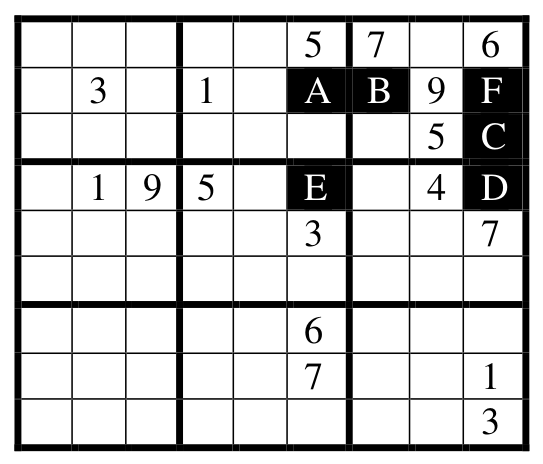
\includegraphics[width=.5\textwidth]{sudoku}%
    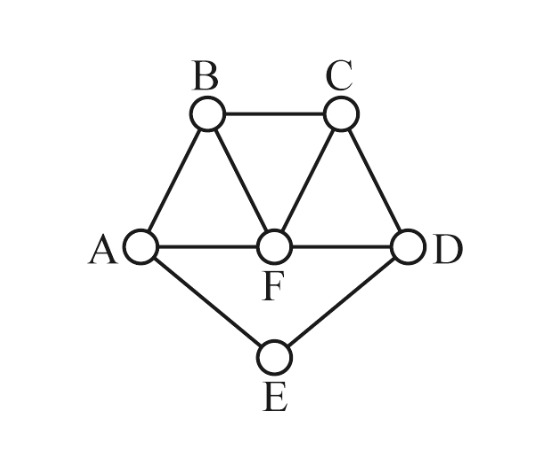
\includegraphics[width=.5\textwidth]{graphe-sudoku}%
  \end{figure}
  
  Les cases A, B, C, F ne peuvent recevoir que 2, 4, ou 8;

  Les cases E et D, que 2 ou 8.  
  
  Peut-on affecter un seul chiffre aux cases A et C ?
  
  }
  
\end{frame}

% ----------------------------------------------------------------------
\begin{frame}<beamer>
  \frametitle{Sommaire}
  \tableofcontents[sections={2-5}]
\end{frame}

% ----------------------------------------------------------------------
\section{Algorithme glouton}
% ----------------------------------------------------------------------

% ----------------------------------------------------------------------
\begin{frame}
  \frametitle{Principe de l'algorithme glouton}

  Réaliser un choix localement optimal à chaque étape en espérant atteindre
  l'optimal global à la fin.

  ~
  
  La plupart du temps, on n'atteint pas l'optimum global, mais pour certains
  problèmes si et pour d'autres, on peut garantir une certaine proximité. 

  % Chvatal : coloration de graphe sans P4
  
  % Claire Mathieu
  % Effectiveness of Local Search for Geometric Optimization
  % Local search yields approximation schemes for k-means and k-median in Euclidean and minor-free metrics

  ~
  
  L'algorithme est souvent facile à implémenter et s'exécute souvent rapidemment. 
  
\end{frame}

% ----------------------------------------------------------------------
\begin{frame}
  \frametitle{Résolution gloutonne du problème d'affectation}

  \[
  C := \left(
  \begin{array}{cccc}
    8 & 3 & 1 & 5 \\
    11 & 7 & 1 & 6 \\
    7 & 8 & 6 & 8 \\
    11 & 6 & 4 & 9 
  \end{array}
  \right)
  \]

  ~
  
  \begin{itemize}
  \item on traite les ouvriers dans un certain ordre ; 
  \item pour chaque ouvrier, on lui affecte la tâche encore disponible de moindre coût.
  \end{itemize}

  ~
  
  \begin{itemize}
  \item $c_{1,3} = 1$, $c_{2,4} = 6$, $c_{3,2} = 8$, $c_{4,1} = 11$.
  \item coût total : $1 + 6 + 8 + 11 = 26$. Optimal ?
  \end{itemize}
  
\end{frame}

% ----------------------------------------------------------------------
\begin{frame}
  \frametitle{Résolution gloutonne de la coloration}


  \begin{figure}[htbp]
    \includegraphics<1>[page=1,width=0.7\textwidth]{ex-graphe}%
    \includegraphics<2>[page=3,width=0.7\textwidth]{ex-graphe}%
    \includegraphics<3>[page=4,width=0.7\textwidth]{ex-graphe}%
    \includegraphics<4>[page=5,width=0.7\textwidth]{ex-graphe}%
    \includegraphics<5>[page=6,width=0.7\textwidth]{ex-graphe}%
    \includegraphics<6>[page=7,width=0.7\textwidth]{ex-graphe}%
    \includegraphics<7>[page=8,width=0.7\textwidth]{ex-graphe}%
    \includegraphics<8>[page=9,width=0.7\textwidth]{ex-graphe}%
    \includegraphics<9>[page=10,width=0.7\textwidth]{ex-graphe}%
  \end{figure}
  
  \begin{itemize}
  \item<2-> on traite les noeuds dans un certain ordre ; 
  \item<3-> pour chaque noeud, on lui affecte la couleur possible de plus petit indice. 
  \end{itemize}

  ~
  
  \begin{itemize}
  \item<9> $4$ couleurs au total. Optimal ?
  \end{itemize}

\end{frame}

% ----------------------------------------------------------------------
\begin{frame}
  \frametitle{Ordres possibles}

  \begin{itemize}
  \item random: noeuds triés aléatoirement. 
  \item largest first: noeuds triés par ordre de degré non croissant.
  \item smallest last: L'ordre $v_1,v_2,\dots,v_n$ est tel
    que $v_i$ a le plus petit degré dans le graphe
    ne contenant plus que les sommets $v_1,v_2,\dots,v_i$.
  \item DSATUR: l'ordre est construit en choisissant à chaque étape
    le noeud $v$ qui maximise la saturation (nombre de couleurs différentes
    déjà affectées aux voisins).
  \item \dots
  \end{itemize}
  
\end{frame}

% ----------------------------------------------------------------------
\section{Backtracking}
% ----------------------------------------------------------------------

% ----------------------------------------------------------------------
\begin{frame}
  \frametitle{Backtracking}

  Méthode constructive pour résoudre un problème de décision :
  \begin{itemize}
  \item on traite les variables du problème dans un certain ordre ;
  \item pour une affectation possible d'une variable, on teste récursivement si une solution valide peut être construite à partir de cette affectation partielle. Si ce n'est pas possible, on abandonne et on revient sur les affectations qui auraient été faites précédemment (backtracking).
  \item on répond non si on a tout tenté sans succès, oui si on a trouvé une solution valide. 
  \end{itemize}
  
\end{frame}

% ----------------------------------------------------------------------
\begin{frame}
  \frametitle{Avertissement}

  On ne résoud pas un problème d'optimisation, mais le problème de \emph{décision}
  ou de \emph{recherche} associé.

  ~

  Dans le cas d'une fonction objectif discrète, le backtracking peut être
  utilisé pour voir si on peut faire mieux qu'une première approximation.

  ~
  
  Par ex. sur le problème de coloration précédent on a trouvé une solution
  à 4 couleurs avec l'algorithme glouton. Existe-t-il une coloration à 3 couleurs ?
  
\end{frame}

% ----------------------------------------------------------------------
\begin{frame}
  \frametitle{Construction d'une 3-coloration par backtracking}


  \begin{figure}[htbp]
    \includegraphics<1>[page=1,width=0.7\textwidth]{ex-graphe-backtracking}%
    \includegraphics<2>[page=2,width=0.7\textwidth]{ex-graphe-backtracking}%
    \includegraphics<3>[page=3,width=0.7\textwidth]{ex-graphe-backtracking}%
    \includegraphics<4>[page=4,width=0.7\textwidth]{ex-graphe-backtracking}%
    \includegraphics<5>[page=5,width=0.7\textwidth]{ex-graphe-backtracking}%
    \includegraphics<6>[page=6,width=0.7\textwidth]{ex-graphe-backtracking}%
    \includegraphics<7>[page=7,width=0.7\textwidth]{ex-graphe-backtracking}%
    \includegraphics<8>[page=8,width=0.7\textwidth]{ex-graphe-backtracking}%
    \includegraphics<9>[page=9,width=0.7\textwidth]{ex-graphe-backtracking}%
    \includegraphics<10>[page=10,width=0.7\textwidth]{ex-graphe-backtracking}%
  \end{figure}
  
  \begin{itemize}
  \item on traite les noeuds dans un certain ordre ; 
  \item pour chaque noeud, on teste les couleurs 1, 2 puis 3 ;
  \item on revient en arrière quand les contraintes sont violées.  
  \end{itemize}

  ~
  
  \alert<3,6,8,9>{backtracking !} \only<10>{ensuite ?}
  
\end{frame}

% ----------------------------------------------------------------------
\begin{frame}
  \frametitle{Algorithme et complexité}

\end{frame}

% ----------------------------------------------------------------------
\section{Programmation dyamique}
% ----------------------------------------------------------------------

% ----------------------------------------------------------------------
\begin{frame}
  \frametitle{Programmation dynamique}

  Il s'agit de décomposer le problème en sous-problèmes, puis résoudre les sous-problèmes,
  des plus petits aux plus grands en stockant les résultats intermédiaires.

  ~
  
  Cette approche est théorisée et nommée ``programmation dynamique'' (pour faire bien)
  par Richard Bellman dans les années cinquantes. Il repose sur la simple observation
  qu'un chemin optimal est formé de sous-chemins optimaux.
  %(ce qui est appelé maintenant principe d'optimalité de Bellman). 

  ~
  
\end{frame}
  
% ----------------------------------------------------------------------
\begin{frame}
  \frametitle{Retour sur le problème d'affectation}

  Il y a $4$ ouvriers et tâches. Pour $k \leq 4$, 

  \[
  (Aff_k) \left\{
  \begin{array}{c}
    \min \ f_k(s) \ \text{tel que :} \\
    s \in S_k \\
  \end{array}
  \right.
  \]

  \begin{itemize}
  \item $S_k$ est l'ensemble des arrangements de $k$ tâches parmi $4$.  
  \item $f_k : S_k \mapsto \R$ est le coût de l'affectation
    de $k$ tâches aux $k$ premiers ouvriers.   
  \end{itemize}

\end{frame}

% ----------------------------------------------------------------------
\begin{frame}
  \frametitle{Formule de récurrence}

  \[ \min_{s \in S_k} f_k(s) = c_k + \min_{s' \in S_{k-1}} f_{k-1}(s'), \]

  où on note $c_k$ le coût minimal d'affectation à l'ouvrier $k$ de
  l'une des tâches non présentes dans la solution $s$. 
  
\end{frame}


%% % ----------------------------------------------------------------------
%% \section{Backtracking}
%% % ----------------------------------------------------------------------

%% % ----------------------------------------------------------------------
%% \begin{frame}
%%   \frametitle{Principe du backtracking}

%%   C'est un algorithme de recherche de solution et non d'optimisation.

  
%% systématiquement l'ensemble des affectations potentielles du problème. Ils consistent à sélectionner une variable du problème, et pour chaque affectation possible de cette variable, à tester récursivement si une solution valide peut-être construite à partir de cette affectation partielle. Si aucune solution n'est trouvée, la méthode abandonne et revient sur les affectations qui auraient été faites précédemment
  
%% \end{frame}

% ----------------------------------------------------------------------
\section{Branch and bound}
% ----------------------------------------------------------------------



% ----------------------------------------------------------------------
\begin{frame}
  \frametitle{Représentation arborescente et principe de séparation}
  
  \begin{itemize}
  \item $S \supseteq X$ est un ensemble de vecteurs possibles
    %$x^T = (x_1,\dots,x_n)$% et la racine d'un arbre. 
  \item On partitionne $S$ en sous-ensembles $S_{(v)} := \{ (x_1,\dots,x_n) \in S \ | \ x_1 = v \}$ \\
    %$\{ S_{(v)} \}_{v \in D(x_1)}$ 
    selon les valeurs prises par $x_1$ 
    %Ces sous-ensembles sont les fils de $S$ par relation d'inclusion.
  \item Pareil selon $x_2$ et ainsi de suite.
    %Chacun d'eux peut être partionné de la même façon selon $x_2$ et ainsi de suite.
  \end{itemize}

  {
    \centering
    \includegraphics<+>[width=0.9\textwidth,page=1]{arbre}
    \includegraphics<+>[width=0.9\textwidth,page=2]{arbre}
    \includegraphics<+>[width=0.9\textwidth,page=3]{arbre}
    \includegraphics<+>[width=0.9\textwidth,page=4]{arbre}
  }
  
\end{frame}

% ----------------------------------------------------------------------
\begin{frame}
  \frametitle{Principe d'évaluation}

  \begin{itemize}
  \item fonction d'évaluation $e$ : pour tout ensemble $T$ descendant de $S$,
    on choisit $e$ telle que $e(T) \leq \min_{x \in T} f(x)$
  \item si on connait une solution $\bar{x} \in S$ et qu'au noeud $T$ on a
    \[f(\bar{x}) < e(T) \leq \min_{x \in T} f(x) \]
  \item alors $T$ ne contient aucune solution optimale et ses descendants
    ne seront pas énumérés
  \end{itemize}
  
\end{frame}

% ----------------------------------------------------------------------
\begin{frame}
  \frametitle{Séparation-évaluation}

  On résoud (exactement) de nombreux problèmes en combinant ces deux principes
  (\emph{Branch and Bound}).

  Il y a d'innombrables variantes selon :
  \begin{itemize}
  \item la fonction d'évaluation
  \item le choix du noeud à explorer (et donc de la valeur à fixer)
  \item le choix de la variable à partir de laquelle on partitionne le noeud choisi
  \end{itemize}

  %% Note : on combine souvent ce principe avec la méthode des \emph{coupes intégrales}
  %% (\emph{Branch and Cut}). 
  
\end{frame}

% ----------------------------------------------------------------------
\begin{frame}
  \frametitle{Exemple d'un problème d'affectation}

  \only<1>{
  \begin{itemize}
  \item 4 ouvriers $\{1,2,3,4\}$ et 4 tâches $\{1,2,3,4\}$
  \item 1 matrice de coût
    $C := \left(
    \begin{array}{cccc}
      8 & 3 & 1 & 5 \\
      11 & 7 & 1 & 6 \\
      7 & 8 & 6 & 8 \\
      11 & 6 & 4 & 9 
    \end{array}
    \right)$ \\
    par ex. affecter l'ouvrier 4 à la tâche 3 coûte $c_{4,3} = 4$ 
  \item Trouver l'affectation de coût minimal
  \end{itemize}
  }

  \only<2>{
    \begin{itemize}
    \item On peut noter les inconnues et contraintes $x^T = (x_1,x_2,x_3,x_4)$,
      telles que $\forall i \in \{ 1,2,3,4\}, \ x_i \in \{ 1,2,3,4\}$ \\
      ($x_i$ contient le numéro de tâche affectée à l'ouvrier $i$).
      
    \item Pour exprimer la fonction objectif, on peut écrire pour tout $i$
      $x_i := \sum_{j=1}^4 j d_{i,j} = d_{i,1} + 2d_{i,2} + 3d_{i,3} + 4d_{i,4} $ \\
      ($d_{i,j} = 1$ si la tâche $j$ est affectée à l'ouvrier $i$, $d_{i,j} = 0$ sinon).
      
    \item Le problème s'exprime donc comme un (PNE)
      \[
      \left\{
      \begin{array}{c}
        \text{min} \ \sum_{i,j} c_{i,j}d_{i,j} \ \text{tel que :} \\
        \forall i \in \{ 1,2,3,4\}, \ x_i \in \{ 1,2,3,4\} \ \text{et} \ x_i = \sum_{j=1}^4 j d_{i,j} 
      \end{array}
      \right.
      \]
    \end{itemize}
  }
 
\end{frame}

% ----------------------------------------------------------------------
\begin{frame}
  \frametitle{Résolution par séparation-évaluation}

  \begin{itemize}
    \item ensemble des affectations possibles : $S$ ($|S| = 4! = 24$) 
    \item fonction d'évaluation $e$ : on somme les coûts minimaux des tâches non affectées, aux coûts des tâches déjà affectées
    \item choix de l'ouvrier selon lequel on sépare : arbitraire %(variable) 
    \item choix de la tâche à fixer en priorité : celle qui minimise $e$ %(valeur)
  \end{itemize}
\end{frame}

% ----------------------------------------------------------------------
\begin{frame}
  \frametitle{Déroulement de la méthode}

  \only<1>{
    \[
    \left(
    \begin{array}{cccc}
      8         & \alert{3} & \alert{1} & \alert{5} \\
      11        & 7         & 1         & 6 \\
      \alert{7} & 8         & 6         & 8 \\
      11        & 6         & 4         & 9 
    \end{array}
    \right)
    \]

    \[ e(S) = (7 + 3 + 1 + 5) = 16 \]

    \begin{itemize}
    \item $\Rightarrow 16$ minorant du coût minimum
    \item choix de l'ouvrier : $1$ 
    \item choix de la tâche à affecter\dots
    \end{itemize}
  }
  \only<2>{
    \begin{center}
    ouvrier 1 $\leftarrow$ tâche 1
    \end{center}
    \[
    \left(
    \begin{array}{cccc}
      \cancel{8}         & \cancel{3}  & \cancel{1}  & \cancel{5} \\
      \cancel{11}        & 7         & \alert{1} & \alert{6} \\
      \cancel{7}         & 8         & 6         & 8 \\
      \cancel{11}        & \alert{6} & 4         & 9 
    \end{array}
    \right)
    \]
  }
  \only<3,6>{
    \begin{center}
    \alert<6>{ouvrier 1 $\leftarrow$ tâche 2}
    \end{center}
    \[
    \left(
    \begin{array}{cccc}
      \cancel{8}& \cancel{3} & \cancel{1}  & \cancel{5} \\
      11             & \cancel{7} & \alert{1}        & \alert{6} \\
      \alert{7}      & \cancel{8} & 6                & 8 \\
      11             & \cancel{6} & 4                & 9 
    \end{array}
    \right)
    \]
  }
  \only<4>{
    \begin{center}
    ouvrier 1 $\leftarrow$ tâche 3
    \end{center}
    \[
    \left(
    \begin{array}{cccc}
      \cancel{8}& \cancel{3} & \cancel{1}  & \cancel{5} \\
      11             & 7               & \cancel{1}  & \alert{6} \\
      \alert{7}      & 8               & \cancel{6}  & 8 \\
      11             & \alert{6}       & \cancel{4}  & 9 
    \end{array}
    \right)
    \]
  }
  \only<5>{
    \begin{center}
    ouvrier 1 $\leftarrow$ tâche 4
    \end{center}
    \[
    \left(
    \begin{array}{cccc}
      \cancel{8}& \cancel{3} & \cancel{1}  & \cancel{5} \\
      11             & 7               & \alert{1}        & \cancel{6} \\
      \alert{7}      & 8               & 6                & \cancel{8} \\
      11             & \alert{6}       & 4                & \cancel{9} 
    \end{array}
    \right)
    \]
  }
  \begin{itemize}
    \item<2-> $e(S_{(1)}) = 8 + (6 + 1 + 6) = 21$
    \item<3-> \alert<6>{$e(S_{(2)}) = 3 + (7 + 1 + 6) = 17$}
    \item<4-> $e(S_{(3)}) = 1 + (7 + 6 + 6) = 20$
    \item<5-> $e(S_{(4)}) = 5 + (7 + 6 + 1) = 19$
  \end{itemize}
    
\end{frame}

% ----------------------------------------------------------------------
\begin{frame}
  \frametitle{Trace sous forme arborescente}

  {
    \includegraphics<+>[width=1\textwidth,page=1]{ex-bb}
    \includegraphics<+>[width=1\textwidth,page=2]{ex-bb}
  } 
\end{frame}

% ----------------------------------------------------------------------
\begin{frame}
  \frametitle{Résultat}


  \[
  e(S_{(4,3,1,2)}) = 5 + 1 + 7 + 6 = 19
  \]
  
  \[
  \left(
  \begin{array}{cccc}
    8 & 3 & 1 & \alert{5} \\
    11 & 7 & \alert{1} & 6 \\
    \alert{7} & 8 & 6 & 8 \\
    11 & \alert{6} & 4 & 9 
  \end{array}
  \right)
  \]

  \begin{block}{Minimum global}
  \begin{itemize}
    \item ouvrier 1 $\leftarrow$ tâche 4
    \item ouvrier 2 $\leftarrow$ tâche 3
    \item ouvrier 3 $\leftarrow$ tâche 1
    \item ouvrier 4 $\leftarrow$ tâche 2
  \end{itemize}
  \end{block}
\end{frame}

% ----------------------------------------------------------------------
\begin{frame}
  \frametitle{Méthodes de résolution}

  \begin{itemize}
  \item recherche exhaustive (très-très petits problèmes)
  \item \alert{\emph{Branch and Bound}} (séparation-évaluation)
  \item relaxation continue dans certains cas particuliers
  \item méthode des coupes (intégrales, mixtes)
  \item \emph{Branch and Bound} + coupes $=$ \emph{Branch and cut}
  \item programmation par contraintes
  \item méta-heuristiques : \\
      glouton, meilleur voisin, tabou, recuit-simulé, algorithme génétique, colonie de fourmis, \dots
  \end{itemize}
  
\end{frame}


% ----------------------------------------------------------------------
\section{Conclusion}
% ----------------------------------------------------------------------

% ----------------------------------------------------------------------
\begin{frame}<beamer>
  \frametitle{Sommaire}
  \tableofcontents[currentsection]
\end{frame}

% ----------------------------------------------------------------------
\begin{frame}
  \frametitle{Différentes classes de problèmes et d'algorithmes}

  \[
  \text{(P)} \left\{
  \begin{array}{c}
    \text{min} \ f(x) \ \text{tel que :} \\
    g_i(x) \leq 0, \ i \in I = \{1, \dots, m\} \\
    x \in S \subseteq \R^n
  \end{array}
  \right.
  \]

  \begin{itemize}
  \item Optimisation continue ($S = \R^n$)
    \begin{itemize}
    \item sans contrainte ($I = \emptyset$) \\
      \emph{descente de gradient}
    \item avec contraintes ($I \neq \emptyset$) 
      \begin{itemize}
        \item non-linéaires
        \item linéaires \\
        \emph{simplexe, points intérieurs}
      \end{itemize}
    \end{itemize}
  \item Optimisation combinatoire ($S = \Z^n$)\\
    \emph{branch and bound}, \emph{(meta)-heuristiques} 
  \end{itemize}
  
\end{frame}

% ----------------------------------------------------------------------
\begin{frame}
  \frametitle{Pour aller plus loin}

  \begin{itemize}
  \item Théorie de la dualité de Lagrange
  \end{itemize}


  \begin{itemize}
  \item Livre de référence sur les aspects théoriques de l'optimisation
  \end{itemize}

\begin{thebibliography}{alpha}
\bibitem{MM}
Michel Minoux, \emph{Programmation mathématique, Théorie et algorithmes}, Lavoisier, 2eme édition, 2008, 711 pp.
\end{thebibliography}

\end{frame}

\end{document}

